\chapter{Analisis Persoalan dan Rancangan Solusi}

Tujuan utama penulisan bab ini adalah untuk menguraikan rencana penyelesaian masalah implementasi sistem \textit{remote deployment} pada lingkungan \textit{IoT} dengan memanfaatkan \textit{kubernetes}. Bagian ini akan memaparkan proses analisis masalah hingga menjadi solusi.


\section{Analisis}

\subsection{Analisis Permasalahan}
\label{sec:analisis-permasalahan}

Pada lingkungan \textit{IoT}, berbagai perangkat terhubung memainkan peran penting dalam mengumpulkan dan memproses data dari lingkungan sekitarnya. Perangkat ini sering kali terbatas sumber daya, memiliki kapasitas pemrosesan, memori, dan penyimpanan yang minim. Meskipun begitu, ada kebutuhan yang meningkat untuk mengerahkan logika aplikasi yang kompleks secara langsung ke perangkat-perangkat ini untuk meningkatkan efisiensi, mengurangi latensi, dan mendukung operasi \textit{offline} atau semi-\textit{offline}. Masalah utama yang muncul adalah bagaimana secara efisien mengelola dan mengerahkan komponen aplikasi pada skala besar dalam lingkungan yang sangat heterogen dan terbatas sumber daya.

Berdasarkan latar belakang yang telah diuraikan pada \textbf{Bagian \ref{sec:latar-belakang}}, masalah ini dapat diselesaikan dengan menggunakan \textit{remote deployment}. Namun, proses pembuatan layanan agar dapat melakukan \textit{remote deplotment} untuk perangkat yang heterogen menjadi hal yang cukup sulit, perlu dibuat sebuah sistem yang mengatur seluruh proses agar menjadi konsisten dan \textit{well documented}. Sistem ini juga bermanfaat untuk pengguna yang ingin mencoba mengembangkan sistem untuk menambah berbagai fitur kedepannya. Standar ini akan terdiri dari model \textit{deployment} serta layanan orkestrasi untuk membantu proses pengelolaan. Layanan orkestrasi, berperan cukup penting dalam sistem, dengan adanya layanan ini proses pengelolaan perangkat yang heterogen menjadi cukup mudah untuk dilakukan. Selain layanan orkestrasi, \textit{deployment plan} model pun perlu memiliki standar agar dapat digunakan oleh \textit{client} atau \textit{developer}.

Sistem dibuat dengan menyediakan infrastruktur yang berorientasi layanan untuk pengerahan komponen aplikasi yang elastis pada perangkat yang memiliki sumber daya yang terbatas pada IoT dengan skala besar. Sistem harus memiliki dukungan untuk melakukan \textit{deployment} berbasis push, serta mengetahui kondisi dari setiap perangkat. Sistem yang dibuat perlu memiliki cara untuk membuat sebuah resep deployment yang terdiri dari beberapa komponen iot serta
pemrosesan paket aplikasi yang disesuaikan dengan platform perangkat, dan mekanisme skalabilitas untuk mengelola penyebaran ke jumlah perangkat yang besar dengan efisien.

Untuk membuat implementasi dari sistem \textit{remote deployment}, terdapat beberapa rintangan yang perlu diatasi. Rintangan tersebut, dapat dirumuskan ke dalam poin-poin sebagai berikut.

\begin{enumerate}
  \item Kondisi saat ini belum banyak sistem \textit{IoT} yang dibuat dan diorkestrasi menggunakan \textit{kubernetes}
  \item Belum ada \textit{deployment plan} yang dapat mendefinisikan proses \textit{deployment} serta agar \textit{remote deployment} dapat diorkestrasi  dengan menggunakan \textit{kubernetes}
  \item Sistem dapat berjalan meskipun dalam kondisi buruk.
  \item Sistem dapat mengetahui kondisi dari masing masing perangkat serta proses \textit{deployment} yang sedang berjalan.
  \item Sistem dapat melakukan deployment dengan metode \textit{push}, sehingga setiap perangkat yang terhubung akan melakukan proses pembaruan secara otomatis.
\end{enumerate}


\section{Analisis Solusi}

Berdasarkan analisis permasalahan pada \ref{sec:analisis-permasalahan} serta studi literatur, Terdapat tiga alternatif solusi untuk mengatasi permasalahan tesrebut.
Mengembangkan sebuah sistem yang memiliki \textit{reliability} dan \textit{observability} yang baik dengan skalabilitas yang tinggi dengan menggunakan kubernetes dengan \textit{service mesh}. Membuat sistem dengan \textit{reliability} yang baik  menggunakan protokol \textit{MQTT}, serta peningkatan layanan internet pada setiap lingkungan disekitar perangkat \textit{IoT}.

\subsection{Perangkat IoT dibekali dengan Internet yang baik}
Salah satu cara untuk mengatasi masalah ini yaitu dengan menaruh internet yang baik disekitar perangkat \textit{IoT}. Dengan adanya hal ini, proses \textit{reliability} akan tercapai serta sistem juga akan memiliki latensi yang rendah. Namun, cara ini tidak optimal dan membutuhkan biaya yang cukup mahal.

Perlu ditempatkan internet yang baik di sekitar perangkat \textit{IoT} memerlukan biaya yang cukup banyak dan cara ini sepenuhnya bergantung pada kualitas \textit{internet service provider} yang digunakan. Apabila \textit{ISP} sedang mengalami penurunan kualitas dan membuat jaringan menjadi buruk maka cara ini sistem akan langsung \textit{unreliable}.

\subsection{Membuat sistem menggunakan protokol MQTT untuk melakukan pertukaran data}
Akan dibuat suatu sistem yang dapat berkomunkasi menggunakan protokol \textit{MQTT}. Sistem ini terdiri dua komponen, \textit{client} dan \textit{broker}. MQTT \textit{client} berfungsi untuk melkukan \textit{subscribe} ataupun \textit{publish} data ke MQTT \textit{broker}. MQTT \textit{broker} sendiri akan menyimpan data yang dikirim oleh sensor ataupun perangkat \textit{IoT} lainnya (publish) dan memiliki reliability yang sangat tinggi sehingga seberapa burukpun jaringannya akan tetap dapat diterima dengan baik \parencite{mqtt}.

\subsection{Membuat \textit{Smart Home System} berbasis Service Mesh dengan kubernetes}
Untuk membuat suatu sistem yang memenuhi dan menjawab permasalahan yang telah diangkat sebelumnya, dapat dibuat suatu sistem menggunakan kubernetes berbasis service mesh





% \subsection{Arsitektur standar untuk \textit{deployment} pada KubeEdge}
% Untuk membuat arsitektur pada KubeEdge perlu memerlukan beberapa konsiderasi terutama pada bagian \textit{EdgeCore}. Secara konsep arsitektur pada KubeEdge tidak jauh berbeda dari kubernetes pada umumnya, namun terdapat perbedaan cara berkomunkasi dari bagian \textit{cloud} dengan \textit{edge} serta komunikasi antar perangkat \textit{IoT} pada \textit{Edge} yang menggunakan MQTT. Dengan melakukan percobaan \textit{deploy} dengan KubeEdge dan melihat referensi pada \ref{sec:riset-terkait} proses standardiasi arsitektur akan mudah untuk dilakukan

% \subsection{Meningkatkan \textit{device discovery} pada layanan}
% Dengan melakukan integrasi dengan \textit{Service Mesh} proses \textit{device discovery} menjadi lebih mudah untuk dilakukan karena untuk setiap aplikasi yang di\textit{deploy} menggunakan KubeEdge, akan ditambah sebuah \textit{sidecar proxy} untuk proses penerimaan maupun pengiriman \textit{request}. Dengan adanya \textit{sidecar proxy} proses \textit{device discovery} menjadi lebih mudah untuk dilakukan.

% \subsection{Menurunkan \textit{low latency} pada layanan}
% Tantangan utama pada aplikasi yang terintegrasi dengan \textit{service mesh} adalah \textit{latency} akan dijamin bertambah karena adanya \textit{extra hop} yang digunakan saat pengiriman maupun penerimaan request. Untuk mengatasi masalah ini dapat digunakan metode lain untuk implementasi \textit{service mesh} seperti \textit{zero-trust tunnel} ataupun menggunakan \textit{eBPF}
% \subsection{Membuat sistem dengan skalabilitas yang baik}
% Dengan menggunakan kubernetes, khususnya \textit{KubeEdge} dapat dibuat sebuah konfigurasi file \textit{deployment} yang telah memenuhi semua \textit{requirements}. File ini akan menjadi acuan untuk proses \textit{deployment} kedepannya.

% \subsection{Membuat sistem dengan \textit{high availability} dan \textit{fault tolerant}}
% Dengan memanfaatkan keunggulan \textit{rollout} dan \textit{rollback} serta \textit{scaling} untuk \textit{deployment} pada kubernetes. Masalah ini menjadi mudah untuk diatasi karena secara umum kubernetes akan memastikan proses \textit{upgrade} ataupun \textit{downgrade} berjalan terlebih dahulu sebelum mematikan layanan yang lama. Karena pada \textit{IoT} memiliki \textit{spec} perangkat yang rendah, proses \textit{scaling} yang digunakan harus menjadi bagian yang dipertimbangkan

\section{Rancangan Solusi}
\label{sec:rancangan-solusi}

\subsection{Gambaran Umum}
Dengan segala kebutuhan yang sudah dianalisis, maka akan dibuat beberapa komponen penyusun sistem. Rencananya, sistem  akan dibuat menggunakan KubeEdge dan perangkat \textit{IoT} akan dibatasi jumlahnya sebanyak lima dan setiap perangkat akan diasumsikan sebagai \textit{cluster} yang berbeda.

\begin{figure}[h]
  \centering
  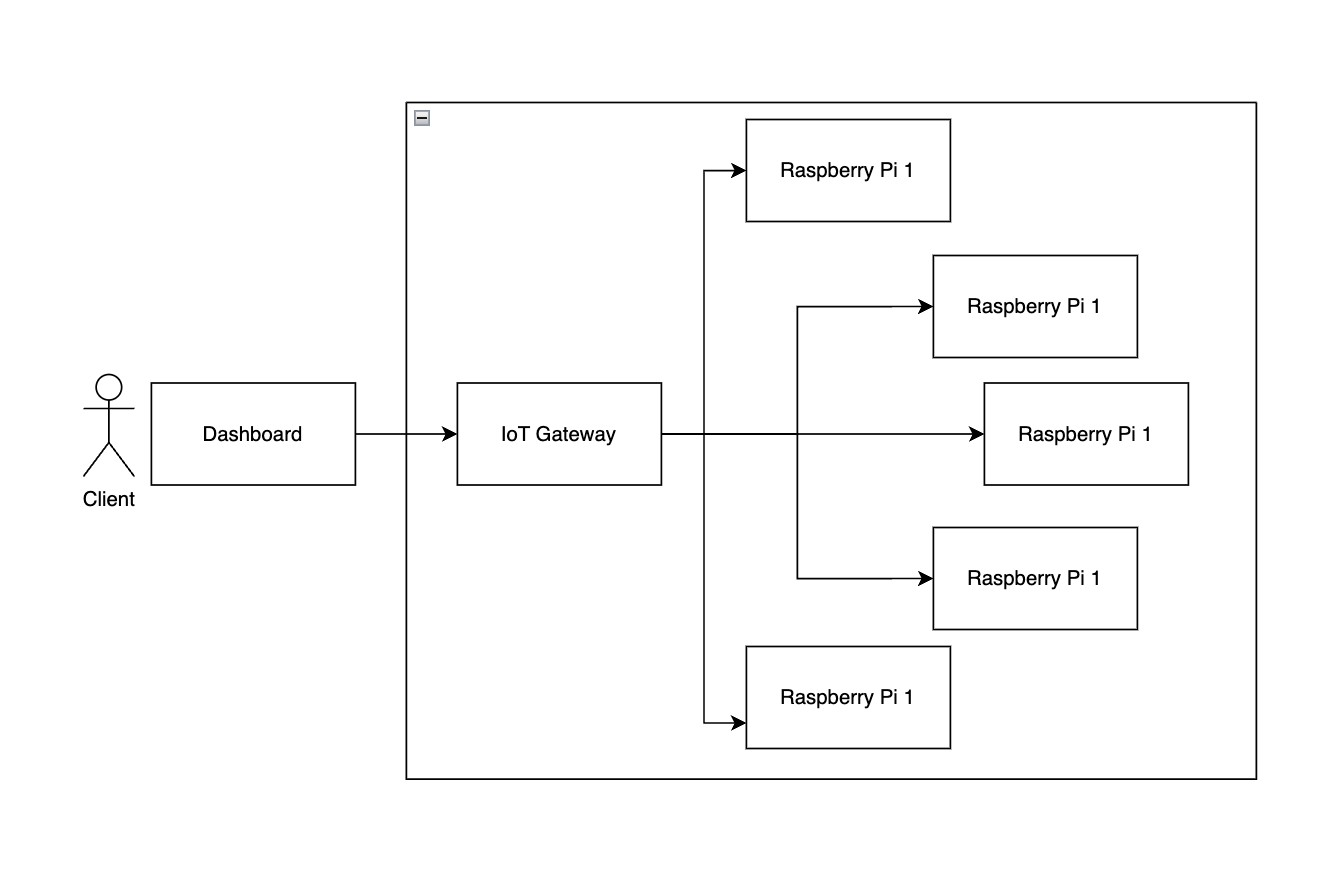
\includegraphics[width=0.5\textwidth]{resources/chapter-3/gambaran-umum-arsitektur.jpg}
  \caption{Gambaran umum arsitektur yang akan dibuat}
  \label{fig:gambaran-umum-arsitektur}
\end{figure}

\section{Rancangan}

\section{Arsitektur Sistem}
Seperti yang telah digambarkan pada \textbf{Gambar \ref{fig:gambaran-umum-arsitektur}}, arsitektur ini memiliki dua komponen utama yang menjadi dasar dari sistem. Yaitu \textit{dashboard} dan \textit{service}. Dashboard memiliki dua modul yaitu modul untuk menampilkan halaman halaman yang bersesuaian dan modul untuk melakukan koneksi dengan \textit{service}.

Service memiliki tiga module yaitu server, database, serta kubernetes. Server akan menjadi pusat kontrol dari \textit{request} yang dikirimkan melalui \textit{dashboard}. Masing masing perangkat akan di \textit{manage} oleh modul kubernetes yang telah memiliki sistem cluster terpisah. Penjelasan arsitektur secara detail akan dijelaskan pada dua subbab yaitu arsitektur struktural serta arsitektur behavioural.

\subsection{Rancangan \textit{Struktural}}
\label{subsec:arsitektur-struktural}

Arsitektur struktural yang digunakan ialah component \textit{diagram}. \textit{component} diagram menggambarkan dengan jelas hubungan antara sistem maupun subsistem yang ada. Sistem digambarkan dengan sebuah box dan module digambarkan dengan persegi panjang yang berada pada dalam box boxnya. Sistem utama dari \textit{remote deployment} hanya terdiri dari \textit{service} dan \textit{dashboard}. Sistem \textit{kubernetes cluster} sepenuhnya di atur oleh modul kubernetes yang ada pada sistem \textit{service}.

\begin{figure}[ht]
  \centering
  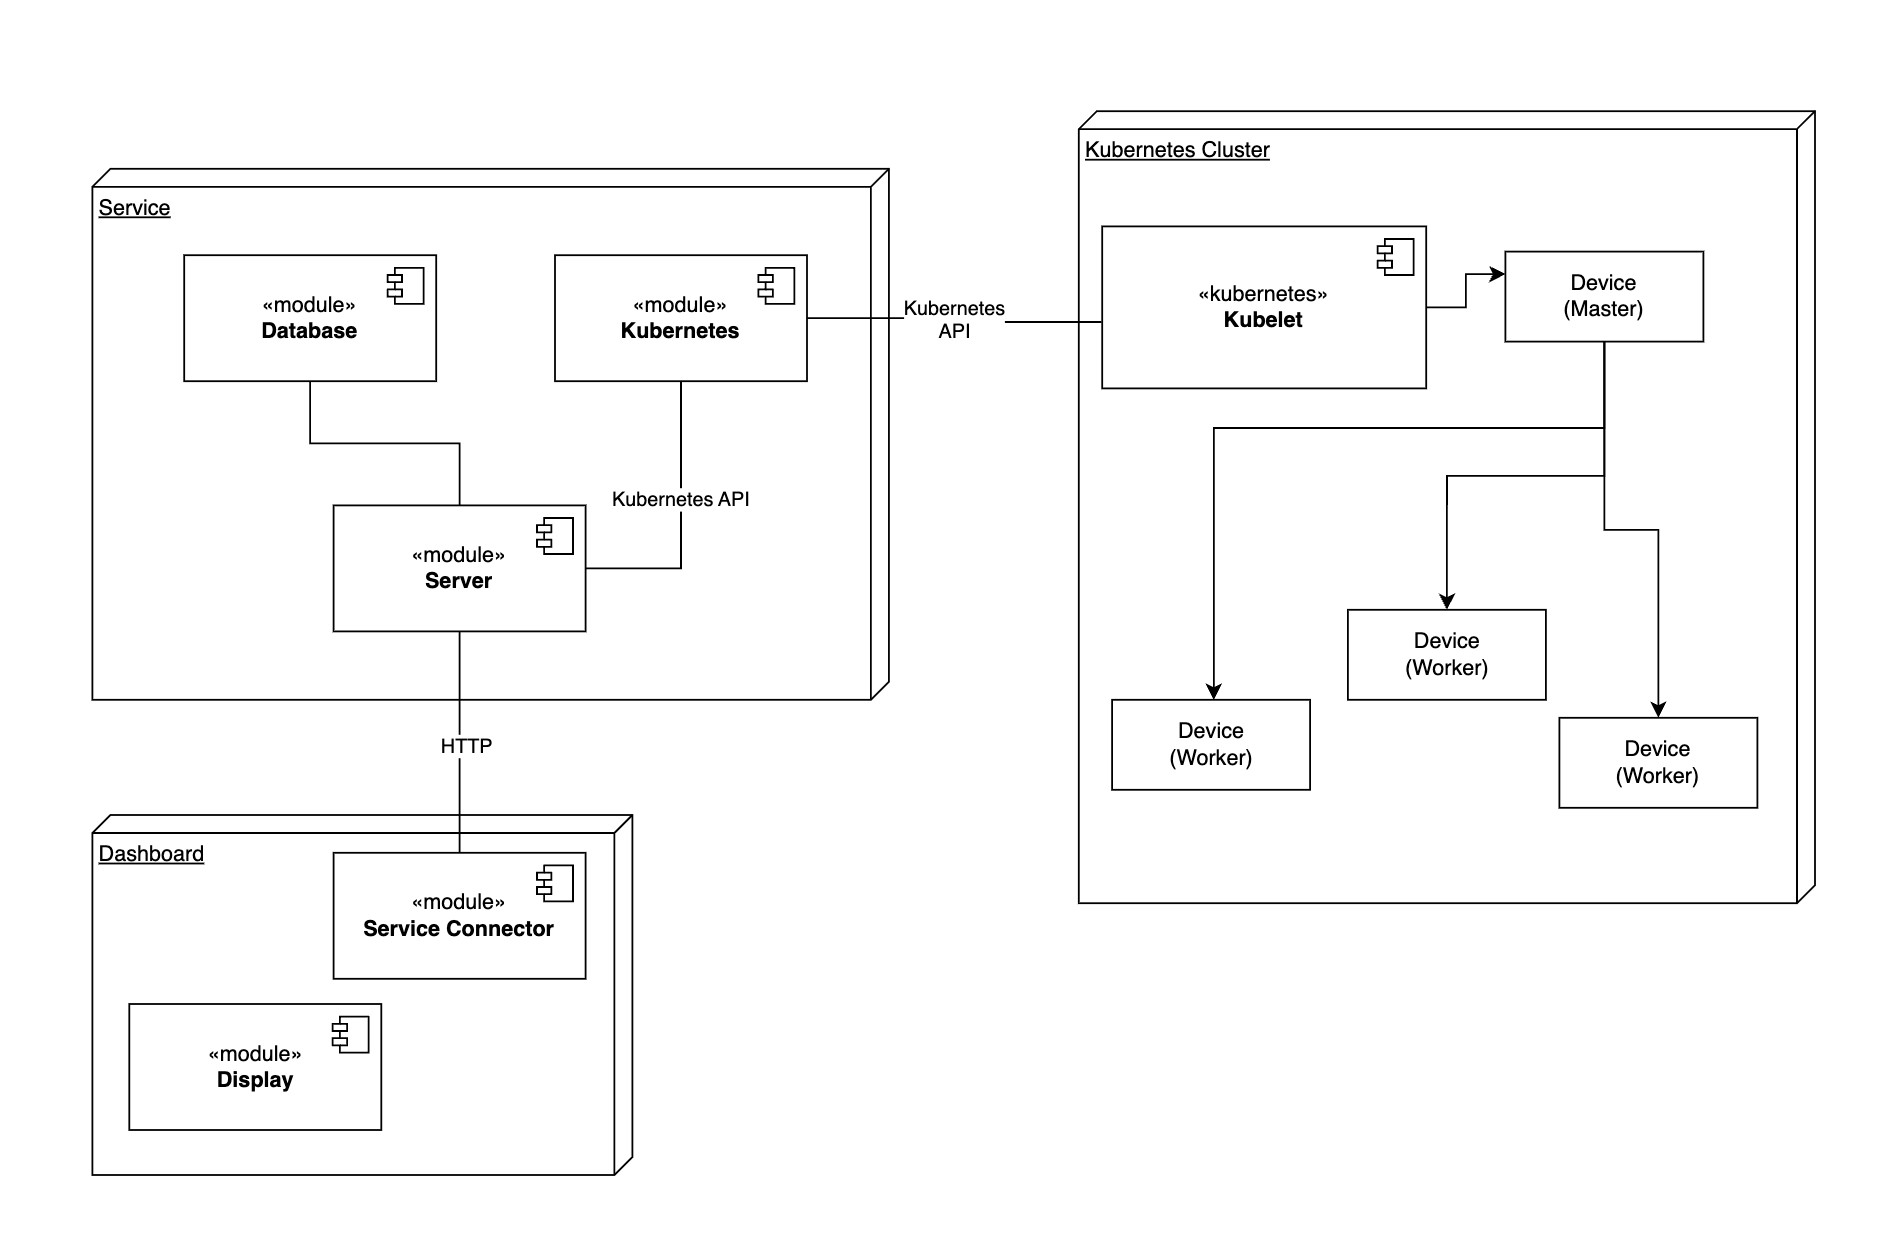
\includegraphics[width=1\textwidth]{resources/chapter-3/package-diagram.jpg}
  \caption{Package Diagram}
  \label{fig:package-diagram}
\end{figure}



\subsection{Rancangan \textit{Behavioural}}
\label{subsec:arsitektur-behavioural}

Berdasarkan \textit{use case} diagram yang telah dibuat, terdapat 13 Use case yang memiliki alur yang berbeda. Untuk menjelaskan interaksi aktor, sistem, serta objek secara terperinci digunakan \textit{sequence} diagram. Terdapat 13 \textit{sequence} pada sistem ini, diagram ini sudah termasuk interaksi antara sistem \textit{dashboard} dan service.

\subsubsection{Alur Mendaftarkan \textit{company}}

Pada \textit{use case} ini, admin yang berperan untuk mendaftarakan \textit{company} baru yang ingin mendaftarkan ke dalam sistem. Admin dapat melakukan request melalui HTTP Client ke server. Server melakukan validasi data dan apabila telah pass, server memasukan informasi ke database. Akhirnya, server memberikan response berupa objek dari \textit{company} yang dapat digunakan. Illustrasi \textit{sequence diagram} dapat dilihat pada gambar \ref{fig:usecase-01}.

\begin{figure}
  \centering
  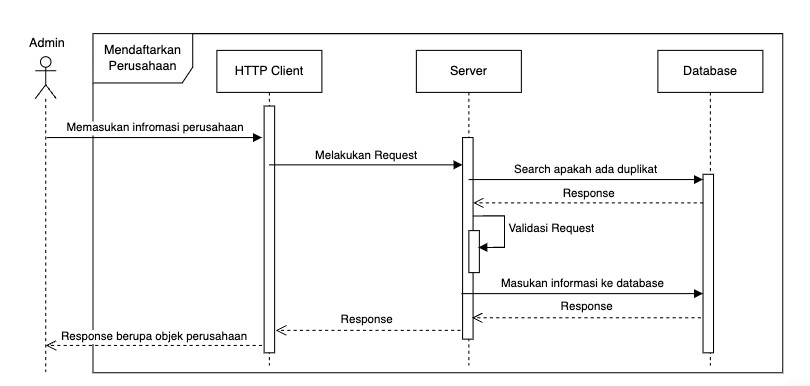
\includegraphics[width=1\textwidth]{resources/chapter-3/usecase/uc-01.jpg}
  \caption{\textit{Use Case} Mendaftarkan \textit{Company}}
  \label{fig:usecase-01}
\end{figure}

\pagebreak

\subsubsection{Alur Mendaftarkan \textit{User}}

Pada \textit{use case} ini, admin yang berperan untuk mendaftarakan \textit{user} baru yang ingin mendaftarkan ke dalam sistem. Admin dapat melakukan request melalui HTTP Client ke server. Server melakukan validasi data dan apabila telah pass, server memasukan informasi ke database. Akhirnya, server memberikan response berupa objek \textit{user} yang dapat digunakan untuk login oleh \textit{user}. Illustrasi \textit{sequence diagram} dapat dilihat pada gambar \ref{fig:usecase-02}.

\begin{figure}[ht]
  \centering
  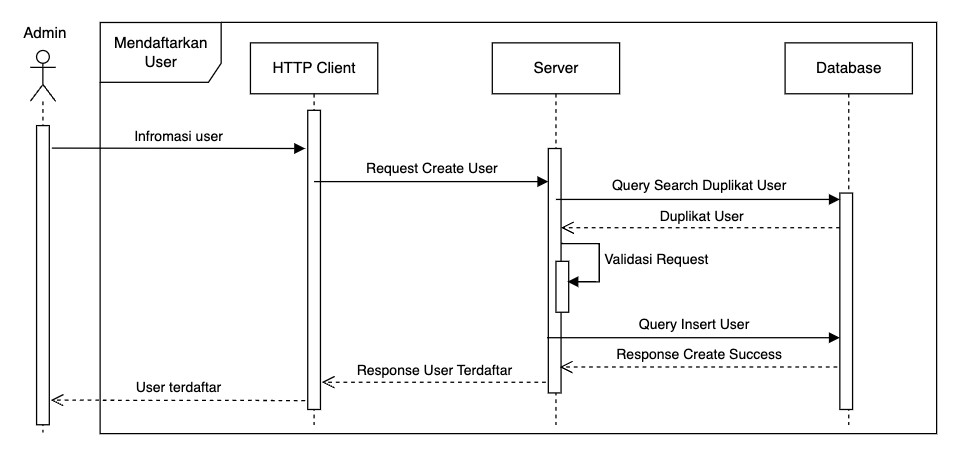
\includegraphics[width=1\textwidth]{resources/chapter-3/usecase/uc-02.jpg}
  \caption{\textit{Use Case} Mendaftarkan \textit{User}}
  \label{fig:usecase-02}
\end{figure}

\subsubsection{Alur Manajemen \textit{company}}

Pada \textit{use case} ini, admin yang berperan untuk melakukan manajemen \textit{company}. Admin dapat menghapus ataupun mengupdate detail \textit{company}. Server melakukan validasi data, setelah melewati seluruh validasi, server melakukan update informasi yang diberikan ke database. Server memberikan repsonse berupa hasil update. Illustrasi \textit{sequence diagram} dapat dilihat pada gambar \ref{fig:usecase-03}.

\begin{figure}[ht]
  \centering
  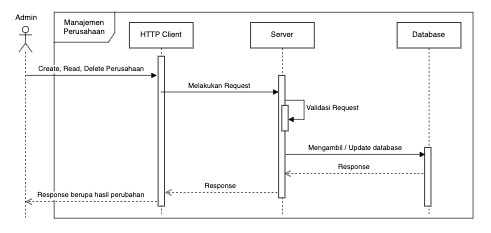
\includegraphics[width=1\textwidth]{resources/chapter-3/usecase/uc-03.jpg}
  \caption{\textit{Use Case} Manajemen \textit{Company}}
  \label{fig:usecase-03}
\end{figure}

\subsubsection{Alur Manajemen \textit{User}}

Pada \textit{use case} ini, admin yang berperan untuk melakukan manajemen \textit{user}. Admin dapat menghapus ataupun mengupdate detail \textit{user}. Server melakukan validasi data dan apabila telah pass, server melakukan update informasi yang diberikan ke database. Setelah itu server memberikan repsonse berupa hasil update yang telah dilakukan. Illustrasi \textit{sequence diagram} dapat dilihat pada gambar \ref{fig:usecase-04}.

\begin{figure}[ht]
  \centering
  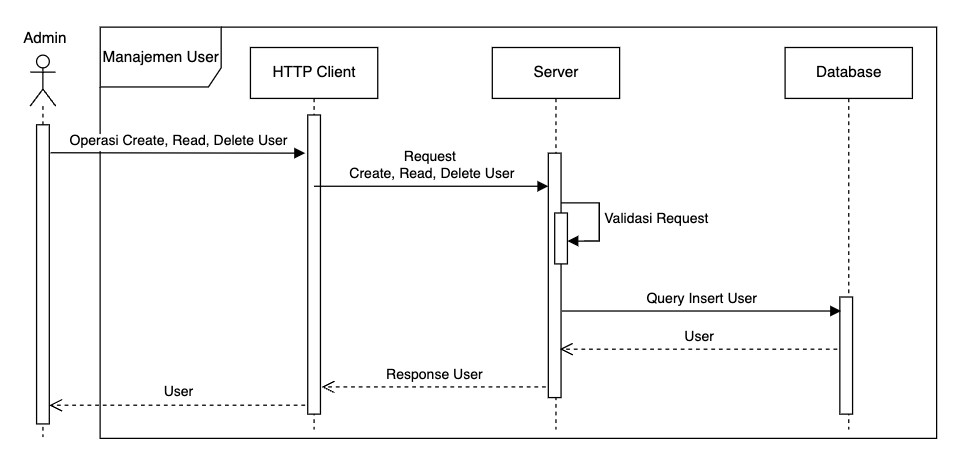
\includegraphics[width=1\textwidth]{resources/chapter-3/usecase/uc-04.jpg}
  \caption{\textit{Use Case} Manajemen \textit{User}}
  \label{fig:usecase-04}
\end{figure}

\subsubsection{Alur Login}

Pada \textit{use case} ini, \textit{user} dapat login ke dalam aplikasi dengan menginput kredensial berupa email dan password. Apabila data yang diberikan tidak valid, muncul modal untuk menandakan kesalahan yang dibuat. Apabila data benar, diberikan modal sukses lalu dilakukan \textit{redirect} ke halaman utama. Pada sisi server, terdapat beberapa validasi seperti apakah email terdapat di database ataupun password match dengan hashed password yang ada di database. Setelah itu, server memberikan response status ok dan memberikan \textit{user} akses ke halaman utama. Illustrasi \textit{sequence diagram} dapat dilihat pada gambar \ref{fig:usecase-05}.

\begin{figure}[ht]
  \centering
  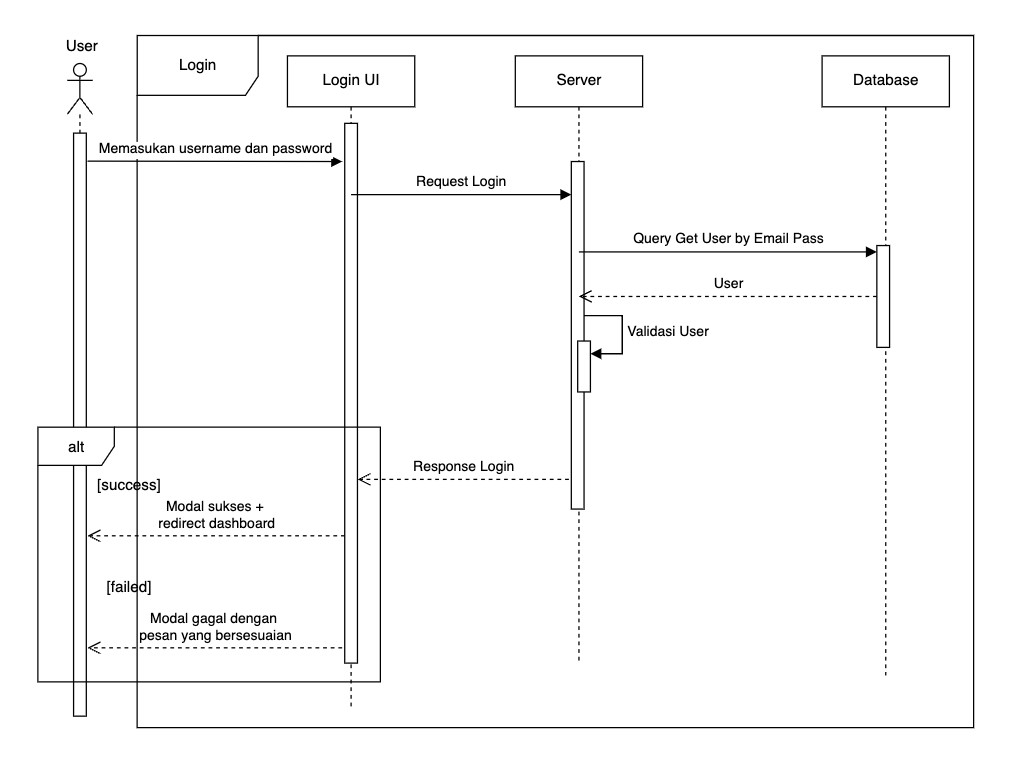
\includegraphics[width=1\textwidth]{resources/chapter-3/usecase/uc-05.jpg}
  \caption{\textit{Use Case} Alur Login}
  \label{fig:usecase-05}
\end{figure}

\subsubsection{Alur Melihat detail \textit{company}}

Pada \textit{use case} ini, \textit{user} dapat melihat detail \textit{company} dengan cara mengunjungi halaman \textit{account}. Data diambil secara langsung melalui \textit{API Call} ke server, apabila terdapat error maka terdapat pesan error yang muncul. Apabila data berhasil di dapatkan, ditampilkan detail dari \textit{company} \textit{user}. Illustrasi \textit{sequence diagram} dapat dilihat pada gambar \ref{fig:usecase-06}.

\begin{figure}[ht]
  \centering
  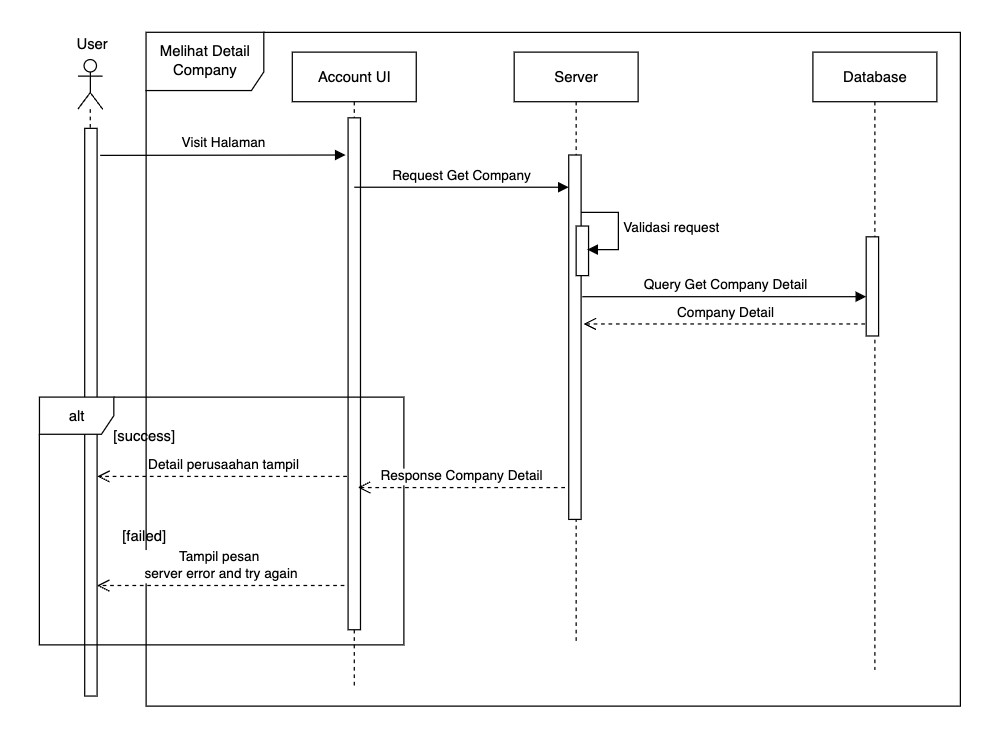
\includegraphics[width=1\textwidth]{resources/chapter-3/usecase/uc-06.jpg}
  \caption{\textit{Use Case} Melihat detail \textit{Company}}
  \label{fig:usecase-06}
\end{figure}

\pagebreak

\subsubsection{Alur Melihat user lain di satu \textit{company}}

Pada \textit{use case} ini, \textit{user} dapat melihat detail seluruh user yang berada pada satu \textit{company} yang sama dengan cara mengunjungi halaman \textit{account}. Data diambil secara langsung melalui API Call ke server, apabila terdapat error maka terdapat pesan error yang muncul. Apabila data berhasil di dapatkan, ditampilkan daftar \textit{user} yang bersesuaian. Illustrasi \textit{sequence diagram} dapat dilihat pada gambar \ref{fig:usecase-07}.


\begin{figure}[ht]
  \centering
  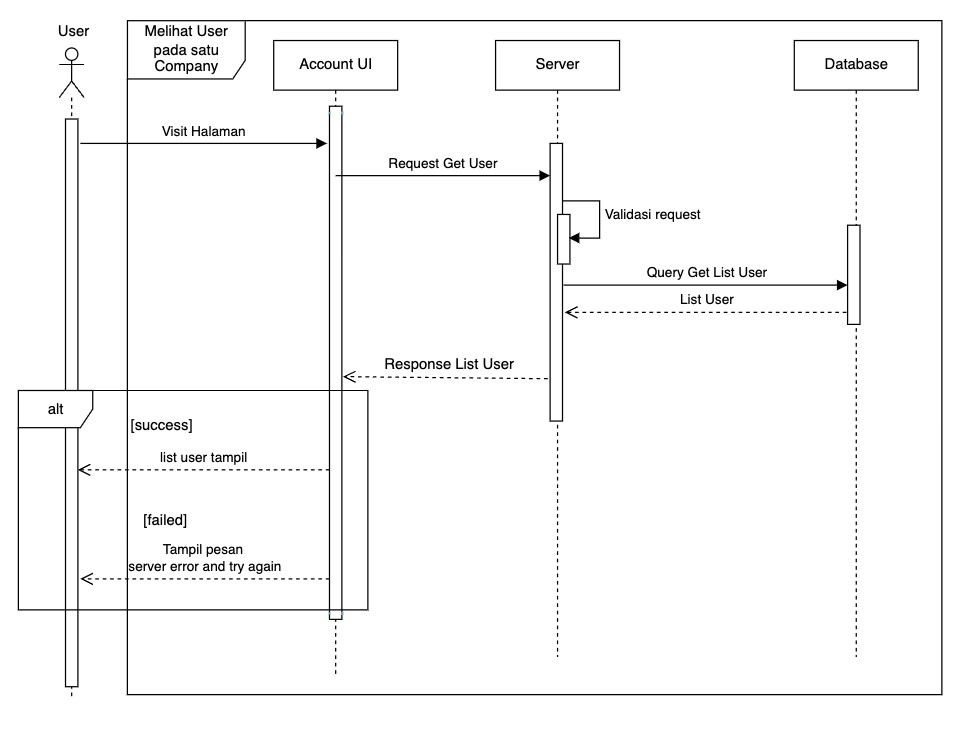
\includegraphics[width=1\textwidth]{resources/chapter-3/usecase/uc-07.jpg}
  \caption{\textit{Use Case} Melihat User Lain pada Satu \textit{Company}}
  \label{fig:usecase-07}
\end{figure}

\pagebreak

\subsubsection{Alur Manajemen \textit{Device}}

Pada \textit{use case} ini, \textit{user} dapat melakuakan manajemen \textit{device} dengan mengunjungi halaman \textit{devices}. Pada halaman ini \textit{user} dapat melakukan beberapa operasi yaitu mengambil daftar \textit{device} yang terdaftar, menambahkan \textit{device} baru, dan menghapus \textit{device}. Operasi pengambilan \textit{device} yang terdaftar dilakukan secara langsung ketika mengunjungi halaman. Operasi penghapusan ataupun penambahan \textit{device} dapat dilakukan oleh \textit{user} dengan cara menekan tombol yang ada pada laman. Ketika tombol ditekan terdapat validasi yang dilakukan pada halaman maupun pada server. Setelah melewati tahapan validasi, server melakukan update pada database. Apabila terdapat error maka terdapat pesan error yang muncul. Apabila data berhasil di dapatkan, ditampilkan sebuah modal yang menandakan operasi berhasil untuk dilakukan. Illustrasi \textit{sequence diagram} dapat dilihat pada gambar \ref{fig:usecase-08}.


\begin{figure}[ht]
  \centering
  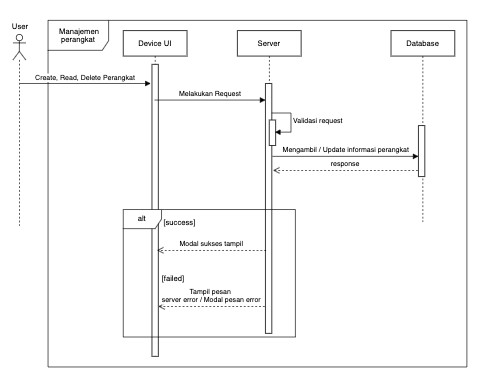
\includegraphics[width=1\textwidth]{resources/chapter-3/usecase/uc-08.jpg}
  \caption{\textit{Use Case} Manajemen \textit{Device}}
  \label{fig:usecase-08}
\end{figure}

\pagebreak

\subsubsection{Alur Manajemen \textit{Groups}}

Pada \textit{use case} ini, \textit{user} dapat melakuakan manajemen \textit{groups} dengan mengunjungi halaman \textit{groups}. Pada halaman ini \textit{user} dapat melakukan beberapa operasi yaitu mengambil daftar \textit{groups} yang terdaftar, menambahkan \textit{groups} baru, dan menghapus \textit{groups}. Operasi pengambilan \textit{groups} yang terdaftar dilakukan secara langsung ketika mengunjungi halaman. Operasi penghapusan ataupun penambahan \textit{groups} dapat dilakukan oleh \textit{user} dengan cara menekan tombol yang ada pada laman. Ketika tombol ditekan terdapat validasi yang dilakukan pada halaman maupun pada server. Setelah melewati tahapan validasi, server melakukan update pada database. Apabila terdapat error maka terdapat pesan error yang muncul. Apabila data berhasil di dapatkan, ditampilkan sebuah modal yang menandakan operasi berhasil untuk dilakukan. Illustrasi \textit{sequence diagram} dapat dilihat pada gambar \ref{fig:usecase-09}.


\begin{figure}[ht]
  \centering
  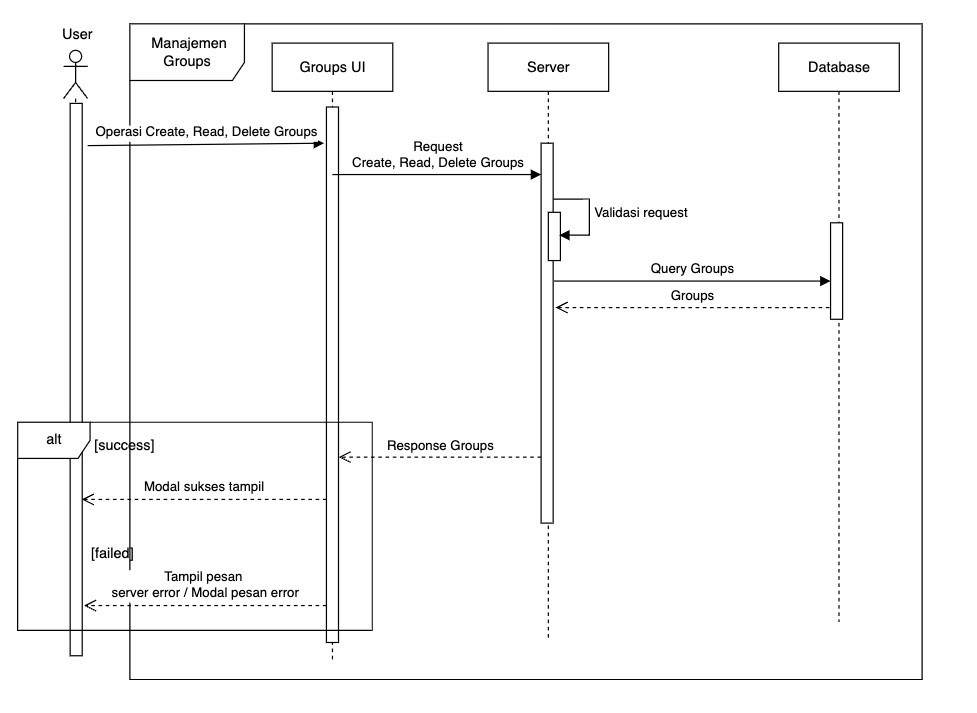
\includegraphics[width=1\textwidth]{resources/chapter-3/usecase/uc-09.jpg}
  \caption{\textit{Use Case} Manajemen \textit{Groups}}
  \label{fig:usecase-09}
\end{figure}

\pagebreak

\subsubsection{Alur Manajemen \textit{Deployment Images}}

Pada \textit{use case} ini, \textit{user} dapat melakuakan manajemen \textit{deployment images} dengan mengunjungi halaman \textit{deployments}. Pada halaman ini \textit{user} dapat melakukan beberapa operasi yaitu mengambil daftar \textit{deployment images}, menambahkan \textit{deployment images} baru, dan menghapus \textit{deployment images}. Operasi pengambilan \textit{deployment images} dilakukan secara langsung ketika membuka halaman. Operasi penghapusan ataupun penambahan \textit{deployment images} dapat dilakukan oleh \textit{user} dengan cara menekan tombol yang ada pada laman. Ketika tombol ditekan terdapat validasi yang dilakukan pada halaman maupun pada server. Setelah melewati tahapan validasi, server melakukan update pada database. Apabila terdapat error maka terdapat pesan error yang muncul. Apabila data berhasil di dapatkan, ditampilkan sebuah modal yang menandakan operasi berhasil untuk dilakukan. Illustrasi \textit{sequence diagram} dapat dilihat pada gambar \ref{fig:usecase-10}.

\begin{figure}[ht]
  \centering
  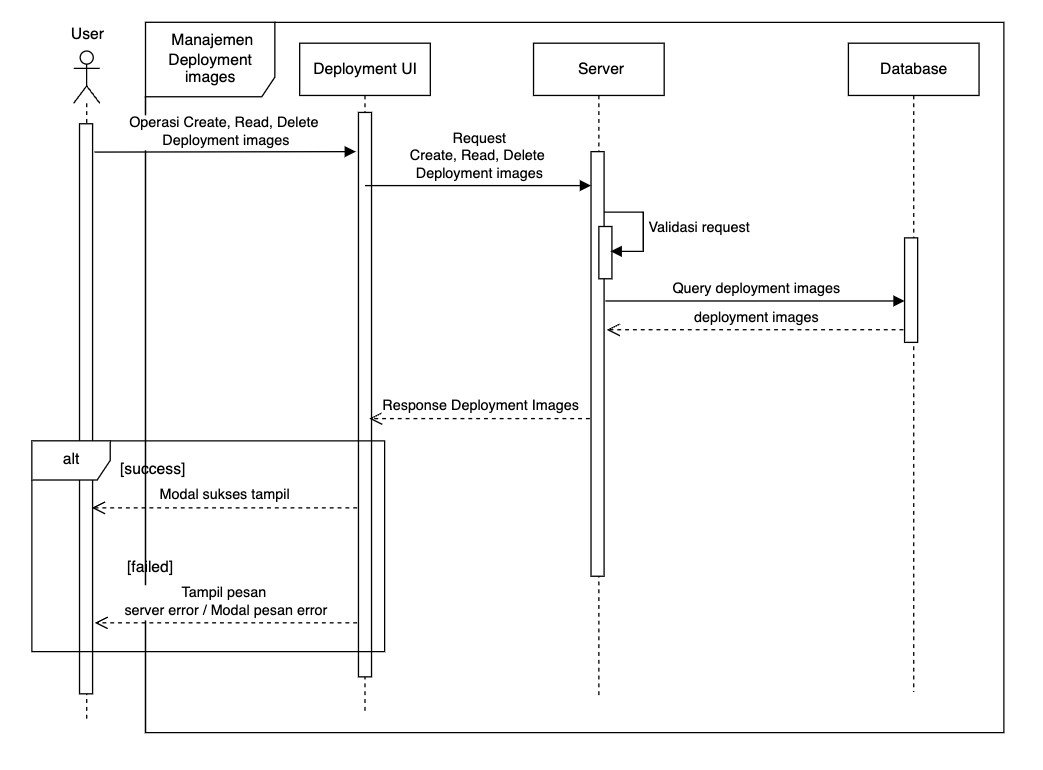
\includegraphics[width=1\textwidth]{resources/chapter-3/usecase/uc-10.jpg}
  \caption{\textit{Use Case} Manajemen \textit{Deployment Images}}
  \label{fig:usecase-10}
\end{figure}

\pagebreak

\subsubsection{Alur Manajemen \textit{Deployment Plan}}

Pada \textit{use case} ini, \textit{user} dapat melakuakan manajemen \textit{deployment plan} dengan mengunjungi halaman \textit{deployments}. Pada halaman ini \textit{user} dapat melakukan beberapa operasi yaitu mengambil daftar \textit{deployment plan} yang terdaftar, menambahkan \textit{deployment plan} baru, dan menghapus \textit{deployment plan}. Operasi pengambilan \textit{deployment plan} yang terdaftar dilakukan secara langsung ketika mengunjungi halaman. Operasi penghapusan ataupun penambahan \textit{deployment plan} dapat dilakukan oleh \textit{user} dengan cara menekan tombol yang ada pada laman. Ketika tombol ditekan terdapat validasi yang dilakukan pada halaman maupun pada server. Setelah melewati tahapan validasi, server melakukan update pada database. Apabila terdapat error maka terdapat pesan error yang muncul. Apabila data berhasil di dapatkan, ditampilkan sebuah modal yang menandakan operasi berhasil untuk dilakukan. Illustrasi \textit{sequence diagram} dapat dilihat pada gambar \ref{fig:usecase-11}.


\begin{figure}[ht]
  \centering
  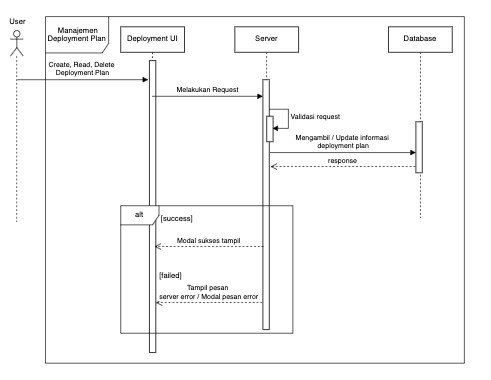
\includegraphics[width=1\textwidth]{resources/chapter-3/usecase/uc-11.jpg}
  \caption{\textit{Use Case} Manajemen \textit{Deployment Plan}}
  \label{fig:usecase-11}
\end{figure}

\pagebreak

\subsubsection{Alur \textit{remote deployment}}

Pada \textit{use case} ini, \textit{user} dapat melakukan \textit{remote deployment} dengan \textit{deployment plan} yang telah dibuat. Aksi ini dilakukan dengan cara mengunjungi halaman \textit{deployments} lalu menekan tombol deploy. Akan ada modal yang muncul memilih deployment yang dilakukan. Ketika user memilih deployment plan yang ingin di \textit{deploy}, terdapat validasi pada server sebelum melakukan deployment pada kubernetes. Setelah semua validasi berhasil dilakukan, kubernetes menginformasikan control plane pada cluster yang terhubung untuk memberikan perintah deploy kepada target. Balikan dari seluruh operasi ini adalah response berupa deployment berhasil dilakukan. Terdapat operasi \textit{asynchronus} pada \textit{background} untuk mengecek status deployment user. Illustrasi \textit{sequence diagram} dapat dilihat pada gambar \ref{fig:usecase-12}.

\begin{figure}[ht]
  \centering
  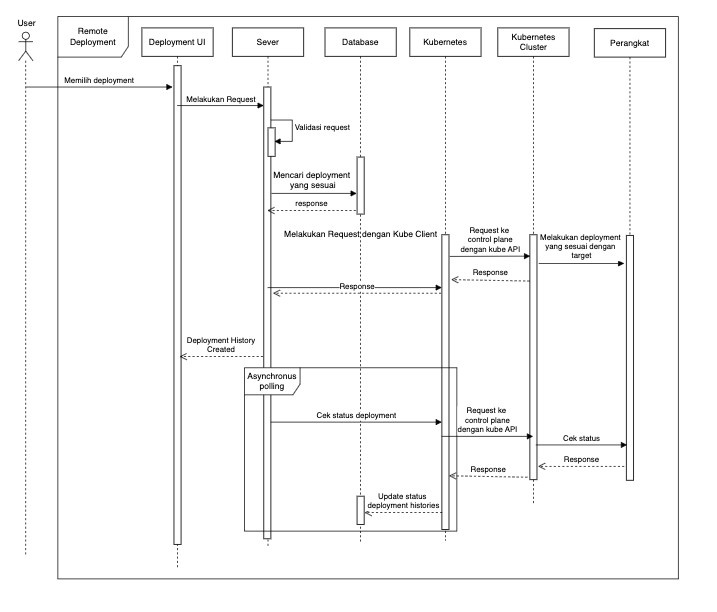
\includegraphics[width=1\textwidth]{resources/chapter-3/usecase/uc-12.jpg}
  \caption{\textit{Use Case} \textit{Remote Deployment}}
  \label{fig:usecase-12}
\end{figure}

\pagebreak

\subsubsection{Alur melihat riwayat \textit{deployment}}

Pada \textit{use case} ini, \textit{user} dapat melihat detail \textit{company} dengan cara mengunjungi halaman \textit{deployments}. Data diambil secara langsung melalui \textit{API Call} ke server, apabila terdapat error maka terdapat pesan error yang muncul. Apabila data berhasil di dapatkan, data menampilkan daftar \textit{deployment} apa saja yang telah dilakukan beserta statusnya. Illustrasi \textit{sequence diagram} dapat dilihat pada gambar \ref{fig:usecase-13}.

\begin{figure}[ht]
  \centering
  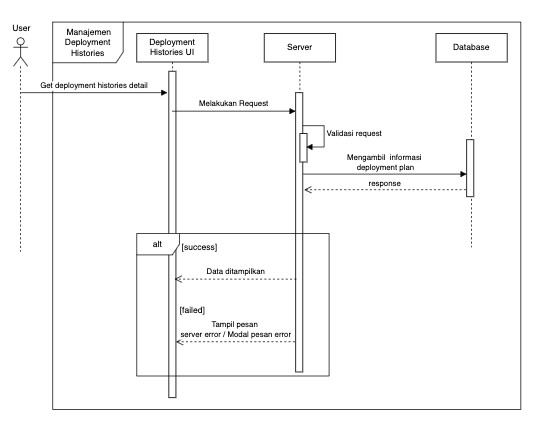
\includegraphics[width=1\textwidth]{resources/chapter-3/usecase/uc-13.jpg}
  \caption{\textit{Use Case} Melihat Riwayat \textit{Deployment}}
  \label{fig:usecase-13}
\end{figure}

\pagebreak

\subsection{Rancangan Detail Komponen Dashboard}
\label{sec:rancangan-dashboard}

Seperti yang telah disebutkan pada bagian \ref{subsec:model-usecase} mengenai \textit{use case} diagram, bagian \ref{subsec:arsitektur-behavioural}, dan bagian \ref{subsec:arsitektur-struktural} dapat dilakukan pemetaan halaman yang dibuat untuk sistem dashboard. Terdapat dua modul yaitu modul \textit{API Connector} serta \textit{display}.

Modul \textit{API Connector} dibuat dengan cara melakukan HTTP Request ke sistem \textit{service}. Modul display yang bertanggung jawab untuk menampilkan halaman yang digunakan oleh user. Pada modul ini terdapat 10 halaman yang dapat dilihat pada daftar di bawah ini.

\begin{enumerate}
  \item Halaman Login

        Halaman ini digunakan sebagai entrypoint dari sistem \textit{dashboard}. Pada halaman ini terdapat beberapa input yang dapat \textit{user} masukan untuk mengirimkan kredensial ke server. Setelah melalui halaman ini, barulah semua fitur dapat diakses.

  \item Halaman utama

        Halaman ini adalah halaman yang dituju oleh \textit{user} ketika telah menyelesaikan proses login. Halaman ini berisi \textit{summary} dari seluruh objek yang terdapat pada perusahaan ini.

  \item Halaman \textit{account}

        Halaman ini adalah halaman yang dapat diakses oleh \textit{user} setelah login. Halaman ini berisi informasi perusahaan \textit{user} serta daftar \textit{user} lain yang terdaftar.

  \item Halaman \textit{devices}

        Halaman ini adalah halaman yang dapat diakses oleh \textit{user} setelah login. Halaman ini berisi informasi mengenai \textit{device} apa saja yang ada pada perusahaan. \textit{user} dapat menghapus serta menambahkan \textit{device} pada halaman ini. Selain itu \textit{user} juga dapat mengunjungi laman detail dari masing masing \textit{device}.

  \item Halaman \textit{devices detail}

        Halaman ini adalah halaman yang dapat diakses oleh \textit{user} setelah login. Halaman ini dapat dituju dengan cara pergi ke halaman \textit{devices} dan memilih \textit{devices} mana yang ingin dilihat informasi lebih lanjut.


  \item Halaman \textit{groups}

        Halaman ini adalah halaman yang dapat diakses oleh \textit{user} setelah login. Halaman ini berisi informasi mengenai \textit{groups} apa saja yang ada pada perusahaan. \textit{user} dapat menghapus serta menambahkan \textit{groups} pada halaman ini. Selain itu \textit{user} juga dapat mengunjungi laman detail dari setiap \textit{groups}.

  \item Halaman \textit{groups detail}

        Halaman ini adalah halaman yang dapat diakses oleh \textit{user} setelah login. Halaman ini dapat dituju dengan cara pergi ke halaman \textit{groups} dan memilih \textit{groups} mana yang ingin dilihat informasi lebih lanjut


  \item Halaman \textit{deployments}

        Halaman ini adalah halaman yang dapat diakses oleh \textit{user} setelah login. Halaman ini berisi informasi mengenai \textit{deployment images} serta \textit{deployment plan} yang ada pada sistem. Selain itu pada halaman ini juga dapat melakukan manajemen serperti menambahkan atau menghapus baik \textit{deployment images} atauapun \textit{deployment plan}. Dari halaman ini pun, dapat diakses detail \textit{deployment images} maupun \textit{deployment plan} serta melakukan \textit{remote deployment}

  \item Halaman \textit{deployments detail}

        Halaman ini menunjukan riwayat \textit{deployment} apa saja yang telah dilakukan, statusnya serta target dari \textit{deployment}.

  \item Halaman \textit{faq}

        Halaman ini bertujuan untuk memberikan informasi mengenai tata cara hal yang perlu dilakukan sebelum mendaftarkan \textit{device} ke sistem


\end{enumerate}

\subsection{Rancangan Detail Komponen Service}
\label{sec:rancangan-service}

Berdasarkan \textit{sequence diagram} yang telah dibuat pada bagian \ref{subsec:arsitektur-behavioural}. Sistem \textit{service} dibagi menjadi beberapa domain. Pembagian domain berfungsi untuk memfokuskan implementasi serta memudahkan tahapan testing. Terdapat 6 domain yaitu \textit{company}, \textit{user}, \textit{devices}, \textit{groups}, \textit{deployment}, dan \textit{external services}. Setiap domain memiliki diagram kelas yang menjelaskan rancangan implementasi. \textit{package} diagram dan \textit{class} diagram secara keseluruhan dapat dilihat pada gambar \ref{fig:package-diagram} dan \ref{fig:package-class-domain-diagram}.
\begin{figure}[ht]
  \centering
  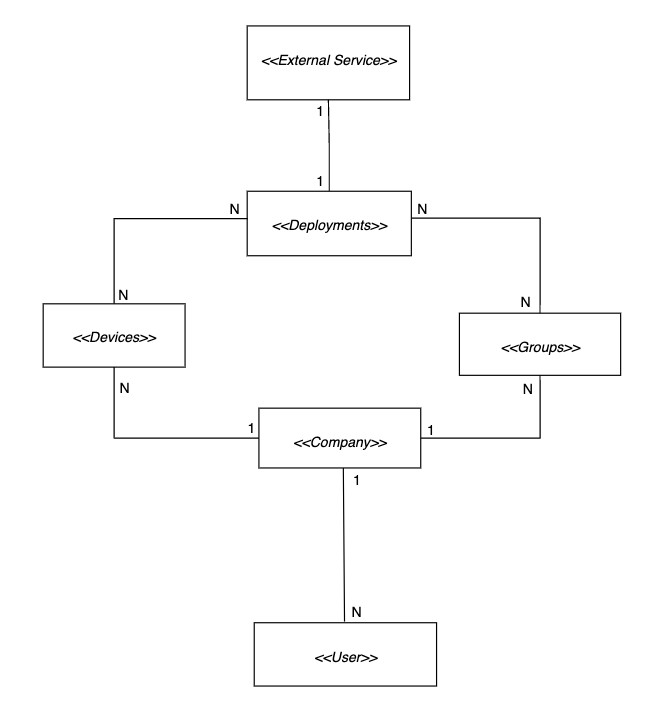
\includegraphics[width=1\textwidth]{resources/chapter-3/class/class-diagram-overall.jpg}
  \caption{\textit{Package Diagram Domain Service}}
  \label{fig:package-class-domain-diagram}
\end{figure}

\pagebreak

\subsubsection{Domain \textit{company}}

Domain ini mengatur konektivitas antara server dan database dalam hal \textit{company}. Domain ini memiliki tiga lapisan yaitu \textit{handler, usecase, dan repository}. Lapisan \textit{repository} memiliki hubungan dengan database serta terdapat lapisan \textit{handler} yang berinteraksi dengan request yang masuk. Illustrasi \textit{class diagram} dapat dilihat pada gambar \ref{fig:company-class-diagram}.

\begin{figure}[ht]
  \centering
  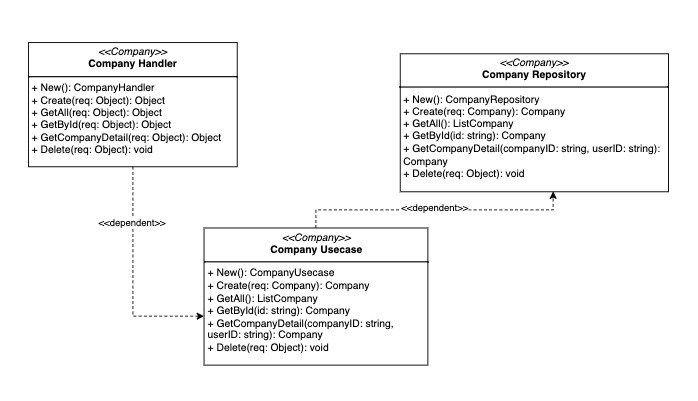
\includegraphics[width=1\textwidth]{resources/chapter-3/class/company-class-diagram.jpg}
  \caption{\textit{Company Class Diagram}}
  \label{fig:company-class-diagram}
\end{figure}

\pagebreak

\subsubsection{Domain \textit{user}}

Domain ini mengatur konektivitas antara server dan database dalam hal \textit{user}. Domain ini juga memliki tiga lapisan mulai dari lapisan paling luar \textit{handler}, diikuti dengan \textit{usecase} lalu terkahir \textit{repository} yang berhubungan dengan database. Domain ini juga yang mengatur bagian autentikasi seperti login dan register. Illustrasi \textit{class diagram} dapat dilihat pada gambar \ref{fig:user-class-diagram}.

\begin{figure}[ht]
  \centering
  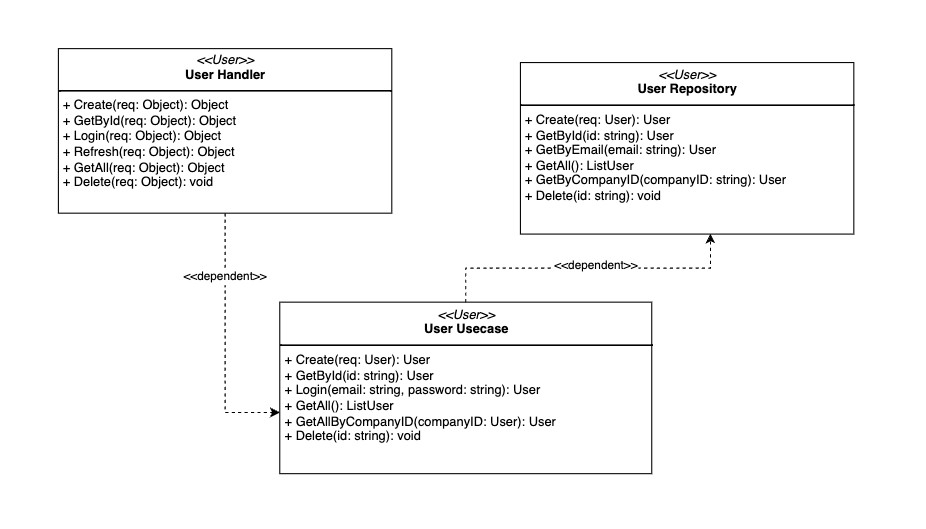
\includegraphics[width=1\textwidth]{resources/chapter-3/class/user-class-diagram.jpg}
  \caption{\textit{User Class Diagram}}
  \label{fig:user-class-diagram}
\end{figure}

\subsubsection{Domain \textit{devices}}

Domain ini mengatur \textit{device} yang ada dalam sistem. Setiap \textit{device} memiliki ikatan dengan \textit{company}. Domain ini mengatur masalah CRUD dari satu \textit{company} yang dapat di \textit{manage} oleh banyak \textit{user}. Sama seperti domain lainnya, domain ini memiliki tiga lapisan yaitu \textit{handler, usecase, dan repository}. Illustrasi \textit{class diagram} dapat dilihat pada gambar \ref{fig:device-class-diagram}.

\begin{figure}[ht]
  \centering
  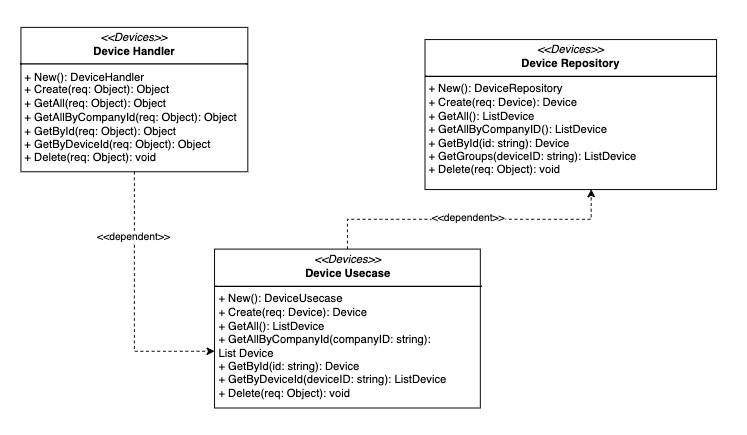
\includegraphics[width=1\textwidth]{resources/chapter-3/class/device-class-diagram.jpg}
  \caption{\textit{Device Class Diagram}}
  \label{fig:device-class-diagram}
\end{figure}

\subsubsection{Domain \textit{groups}}

Domain ini mengatur \textit{groups} yang merupakan gabungan dari satu atau lebih \textit{device}. Seperti domain \textit{devices}, domain ini pun dapat dikelompokan berdasarkan \textit{company}. Seluruh \textit{user} dapat manage \textit{groups} selama masih dalam satu perusahaan yang sama. Domain ini juga memiliki tiga lapisan yaitu \textit{handler, usecase, dan repository}. Illustrasi \textit{class diagram} dapat dilihat pada gambar \ref{fig:groups-class-diagram}.

\begin{figure}[ht]
  \centering
  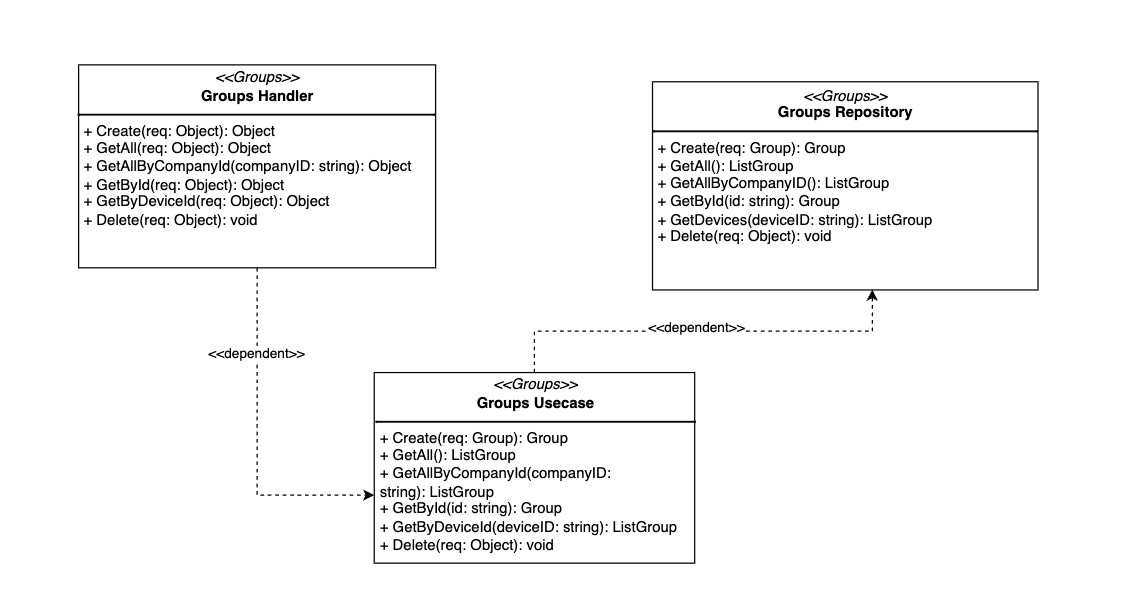
\includegraphics[width=1\textwidth]{resources/chapter-3/class/groups-class-diagram.jpg}
  \caption{Groups \textit{Class Diagram}}
  \label{fig:groups-class-diagram}
\end{figure}

\pagebreak

\subsubsection{Domain \textit{deployment}}

Domain ini merupakan domain yang paling \textit{complex} pada service ini. Domain ini cukup luas karena berhubungan dengan \textit{deployment images} dan \textit{deployment history}. Selain itu domain ini juga memiliki hubungan dengan external service yaitu \textit{kubernetes} untuk proses deploymentnya. Illustrasi \textit{class diagram} dapat dilihat pada gambar \ref{fig:deployment-class-diagram}

\begin{figure}[ht]
  \centering
  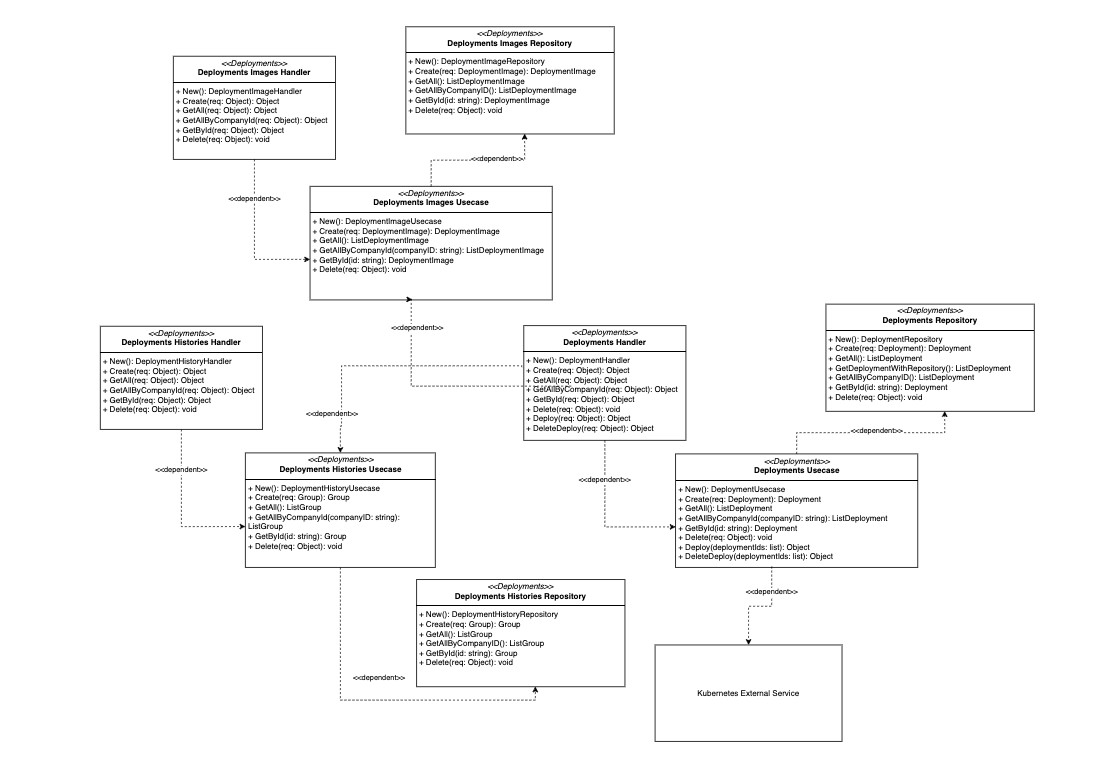
\includegraphics[width=1\textwidth]{resources/chapter-3/class/deployment-class-diagram.jpg}
  \caption{Deployment \textit{Class Diagram}}
  \label{fig:deployment-class-diagram}
\end{figure}

\subsubsection{Domain \textit{external services}}

Domain ini merupakan sebuah interface dari \textit{external service} yang digunakan oleh sistem. Terdapat dua external service yaitu \textit{database} dan \textit{kubernetes}. Namun, hanya \textit{kuberntes controller} saja yang dibuat \textit{class diagram} karena untuk \textit{database} itu sudah diimplementasikan di masing masing domain pada lapisan \textit{repository}. Illustrasi \textit{class diagram} dapat dilihat pada gambar \ref{fig:kubernetes-controller-class-diagram}

\begin{figure}[ht]
  \centering
  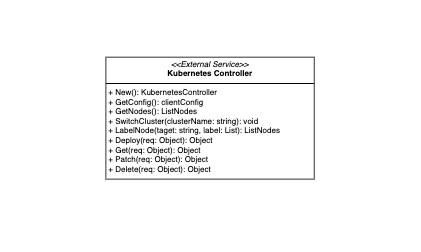
\includegraphics[width=0.7\textwidth]{resources/chapter-3/class/kubernetes-controller}
  \caption{Kubernetes Controller \textit{Class Diagram}}
  \label{fig:kubernetes-controller-class-diagram}
\end{figure}